\chapter{Results with 13 TeV data}
\label{ch:results13}

\section{Final $\mWV$ distribution}

\begin{figure}[htbp]
\centering
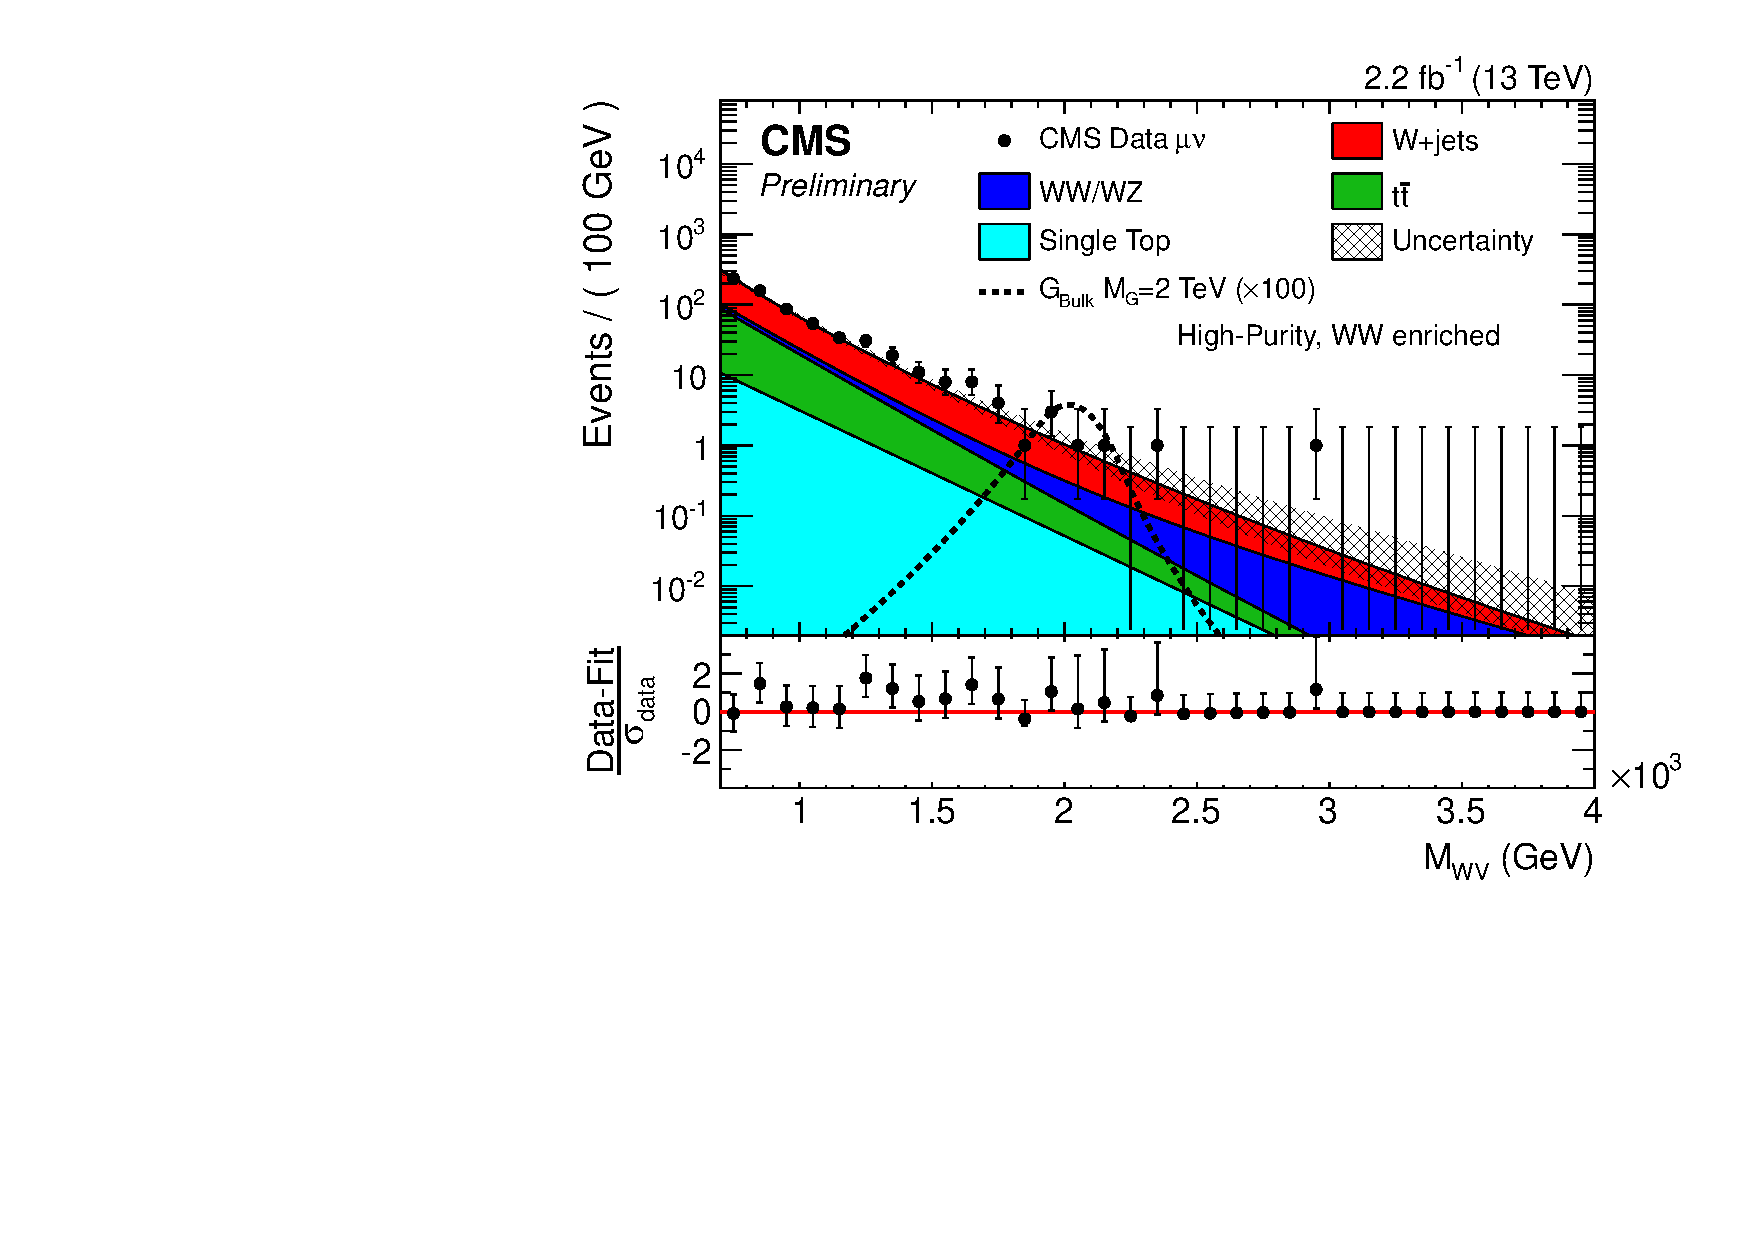
\includegraphics[width=0.48\textwidth]{\chtwelve/HPW_mlvj_fitting_mu}%
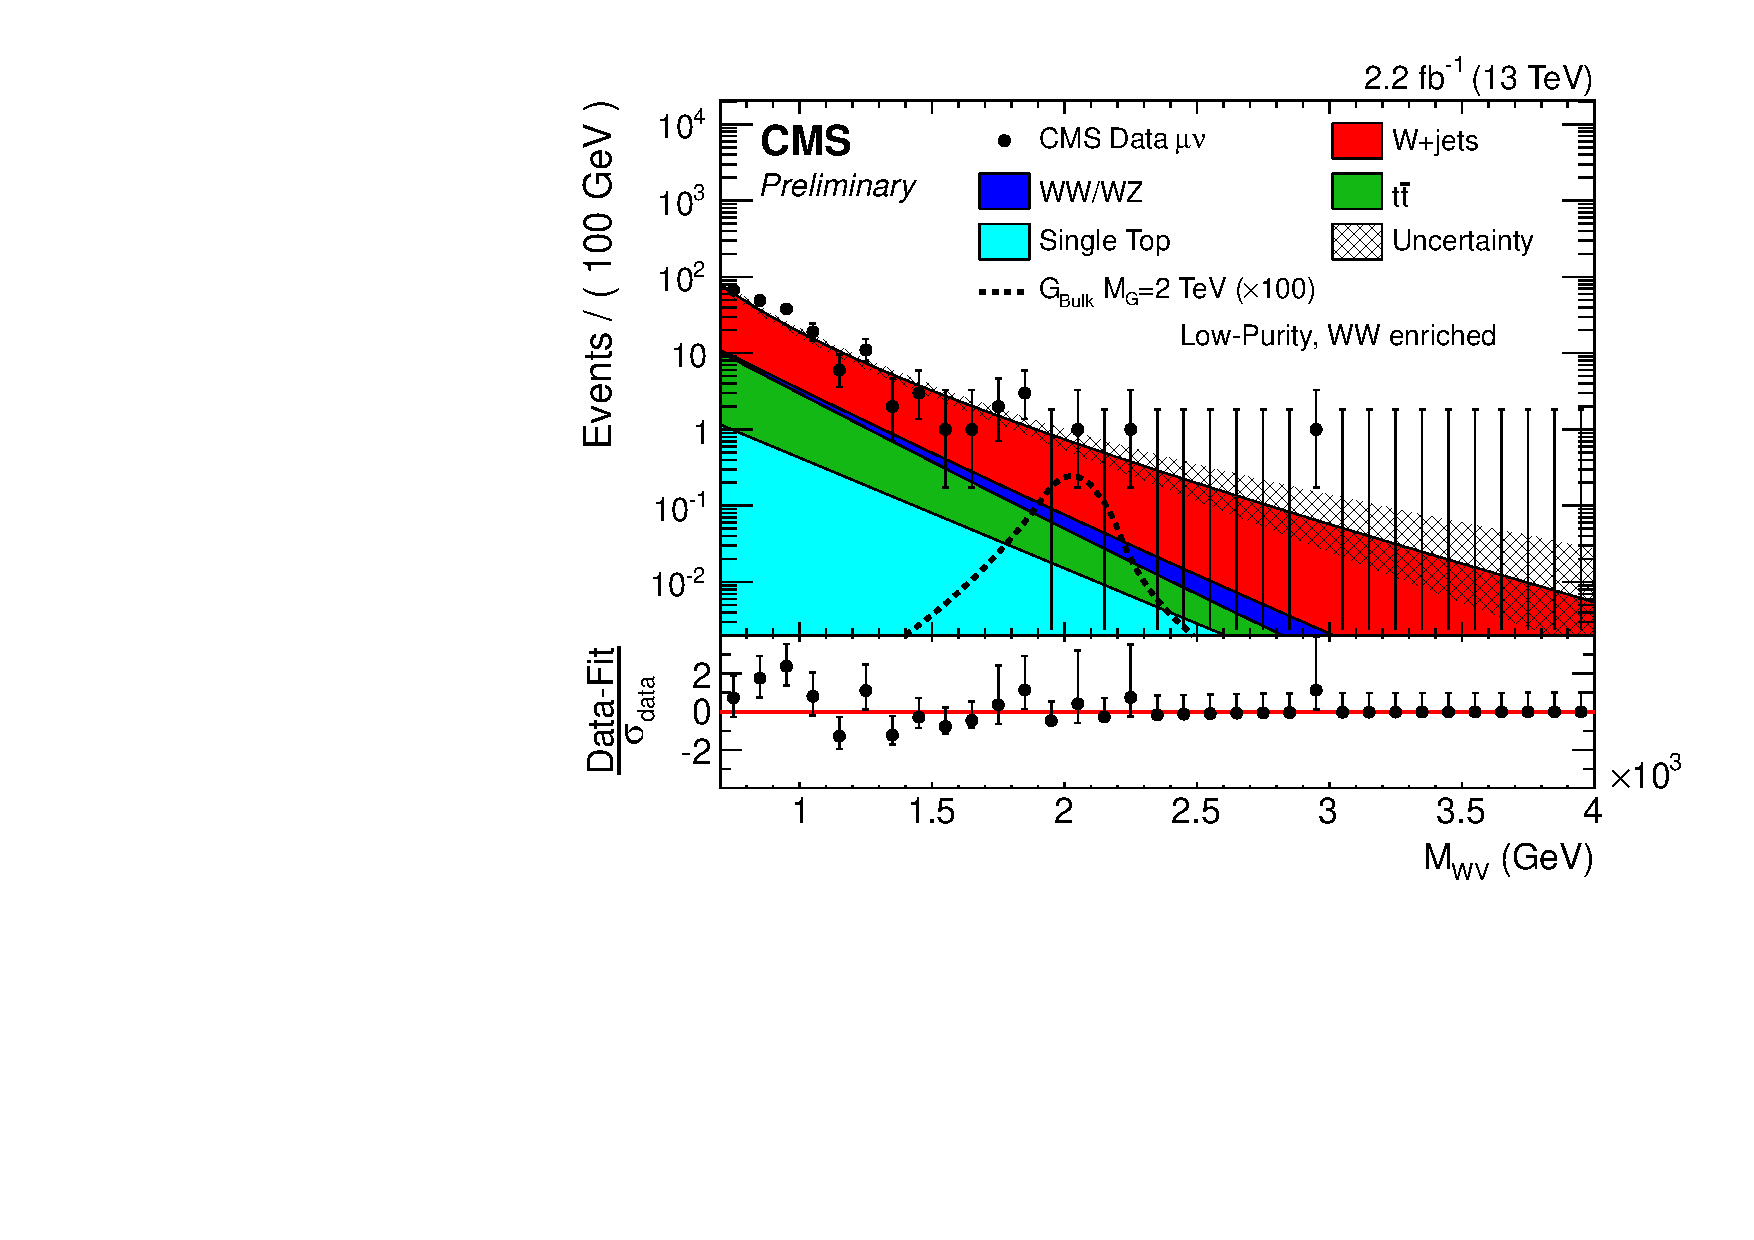
\includegraphics[width=0.48\textwidth]{\chtwelve/LPW_mlvj_fitting_mu}\\
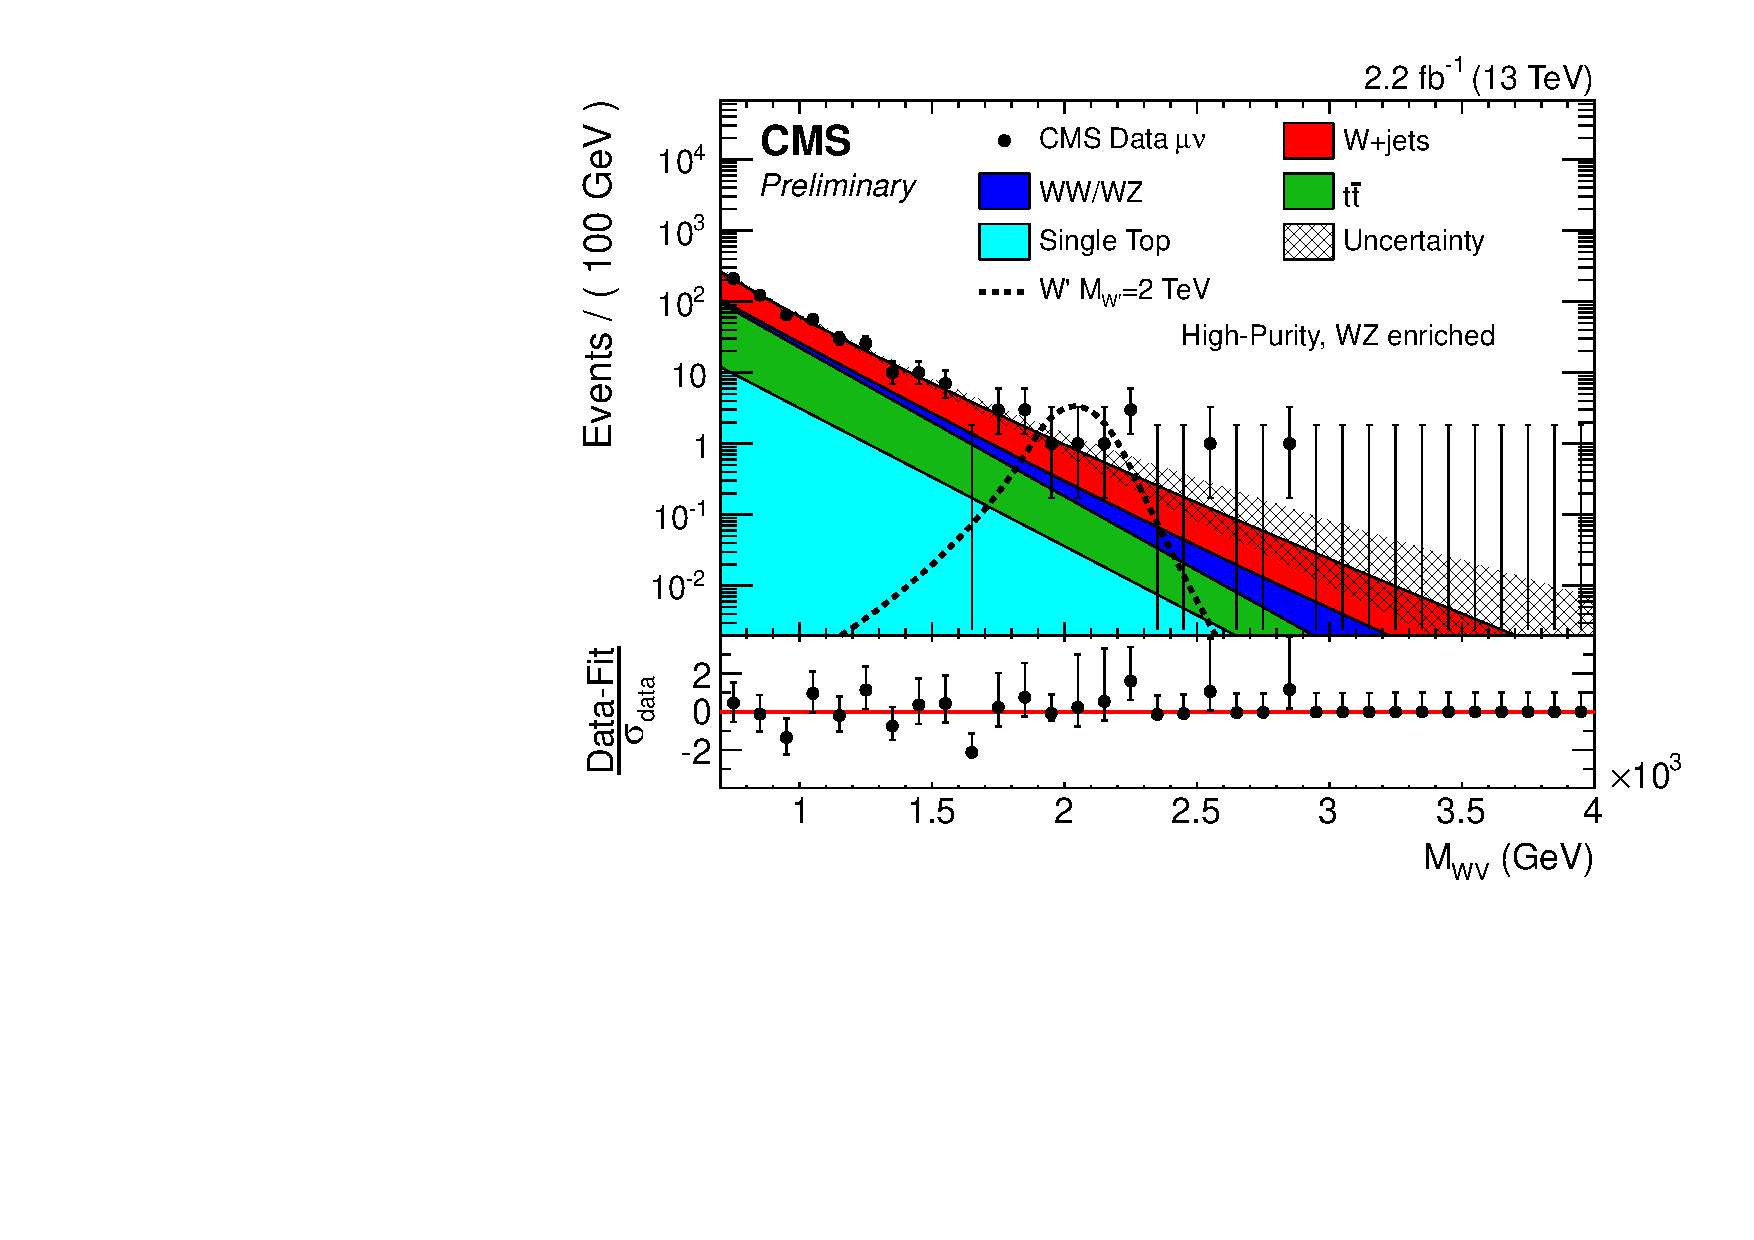
\includegraphics[width=0.48\textwidth]{\chtwelve/HPZ_mlvj_fitting_mu}
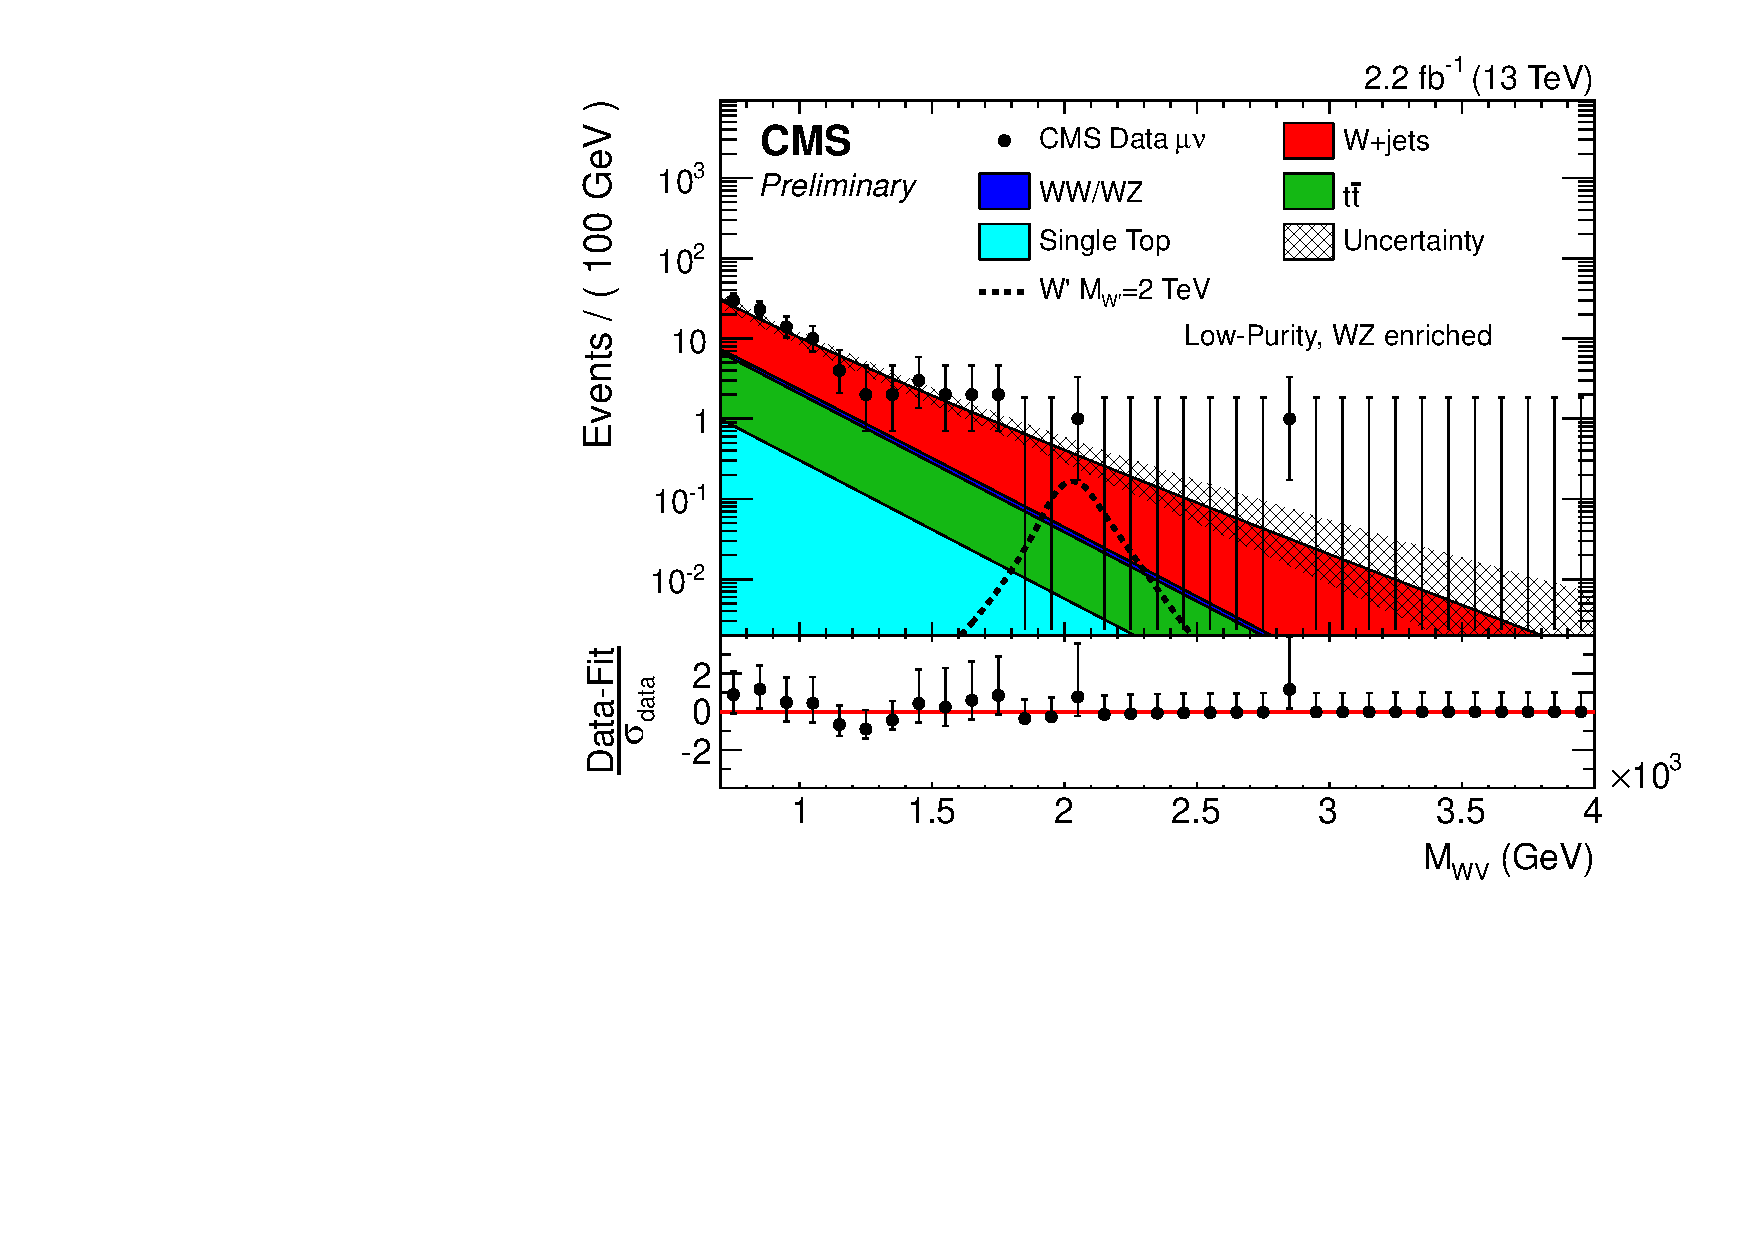
\includegraphics[width=0.48\textwidth]{\chtwelve/LPZ_mlvj_fitting_mu}\\
\caption{Examples of $m_J$ extrapolation of the $m_{\ell\nu j}$ shape into the Signal Region
for the muon channel for the HP (left) and LP (right) categories in the WW (top) and WZ (bottom) signal regions.
The expected shape for a Bulk Graviton and for a W' with a mass of 2 TeV is also shown
in the WW-enriched and WZ-enriched category, respectively.}
\label{fig:srFits_mu}
\end{figure}

\begin{figure}[htbp]
\centering
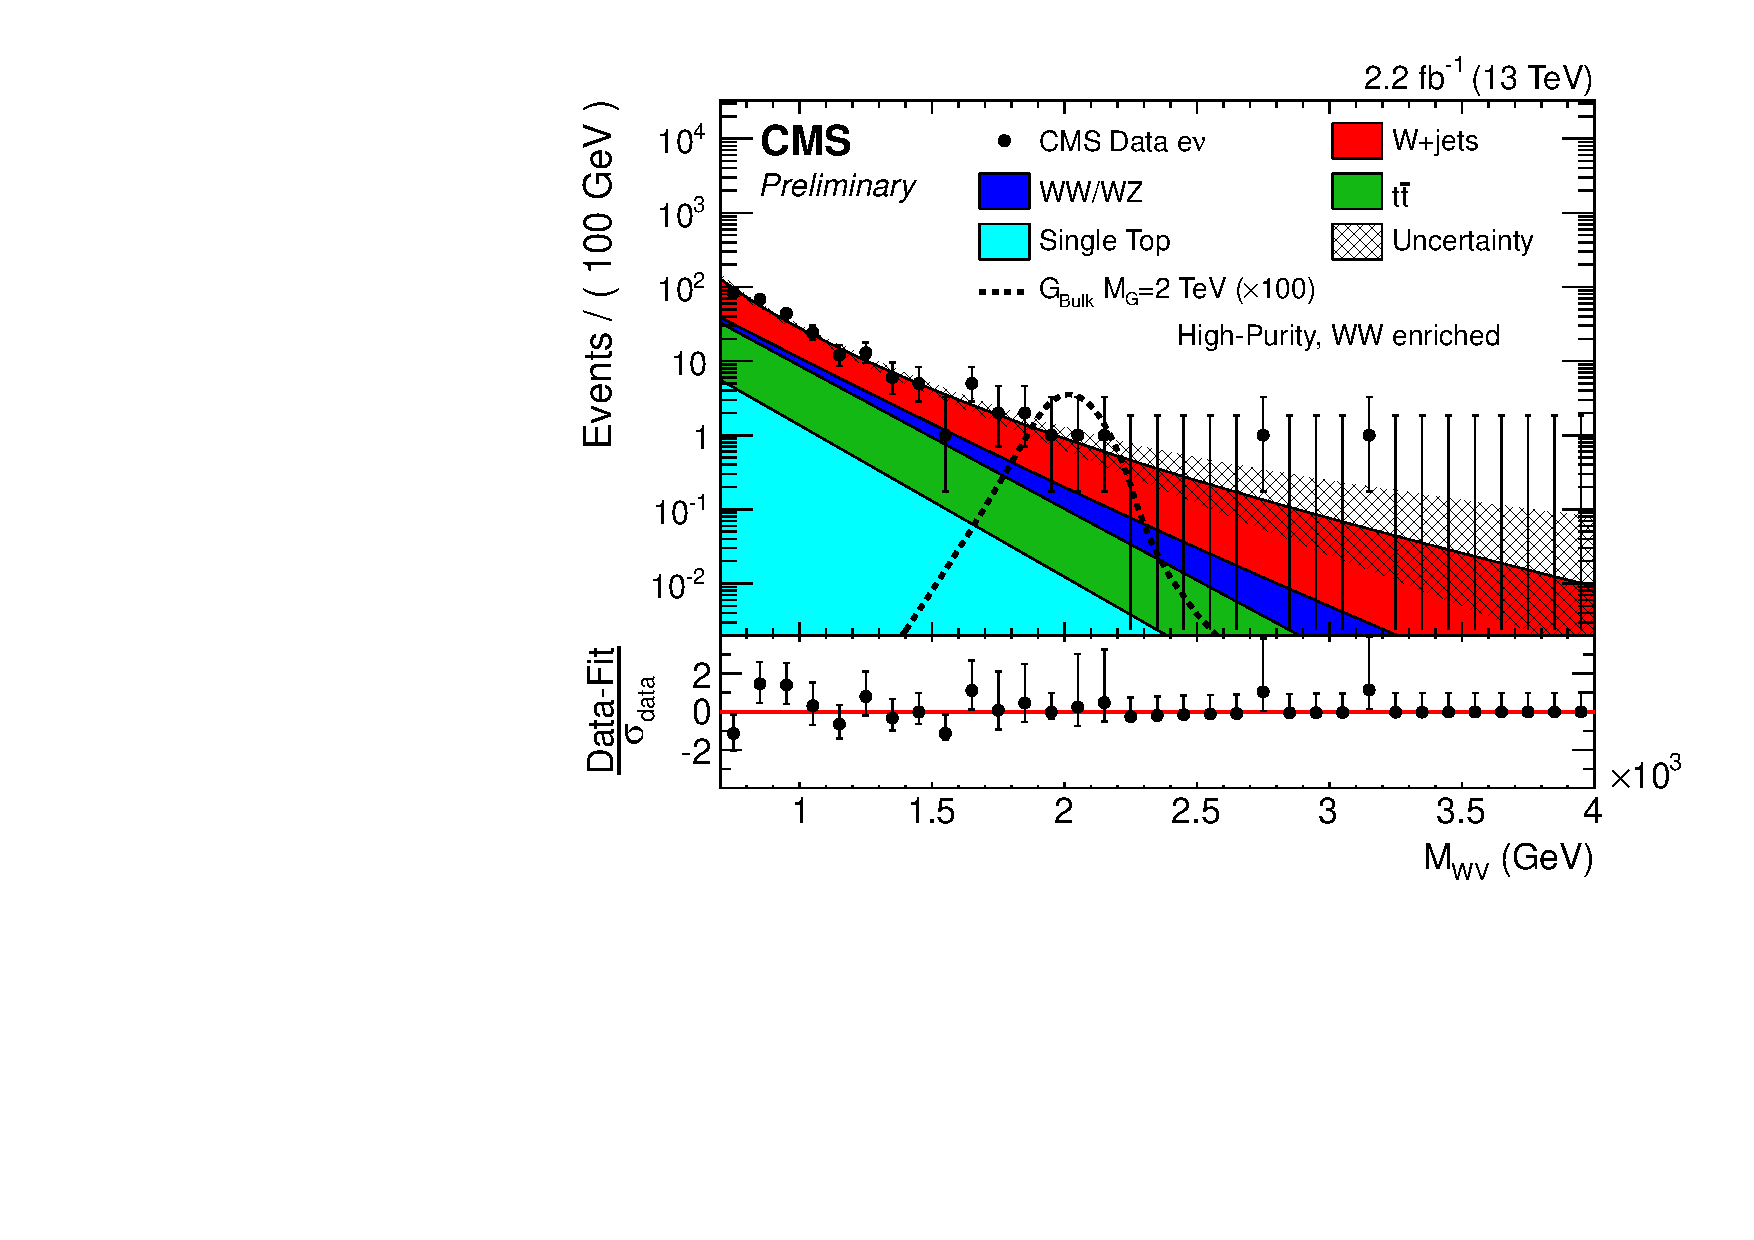
\includegraphics[width=0.48\textwidth]{\chtwelve/HPW_mlvj_fitting_el}%
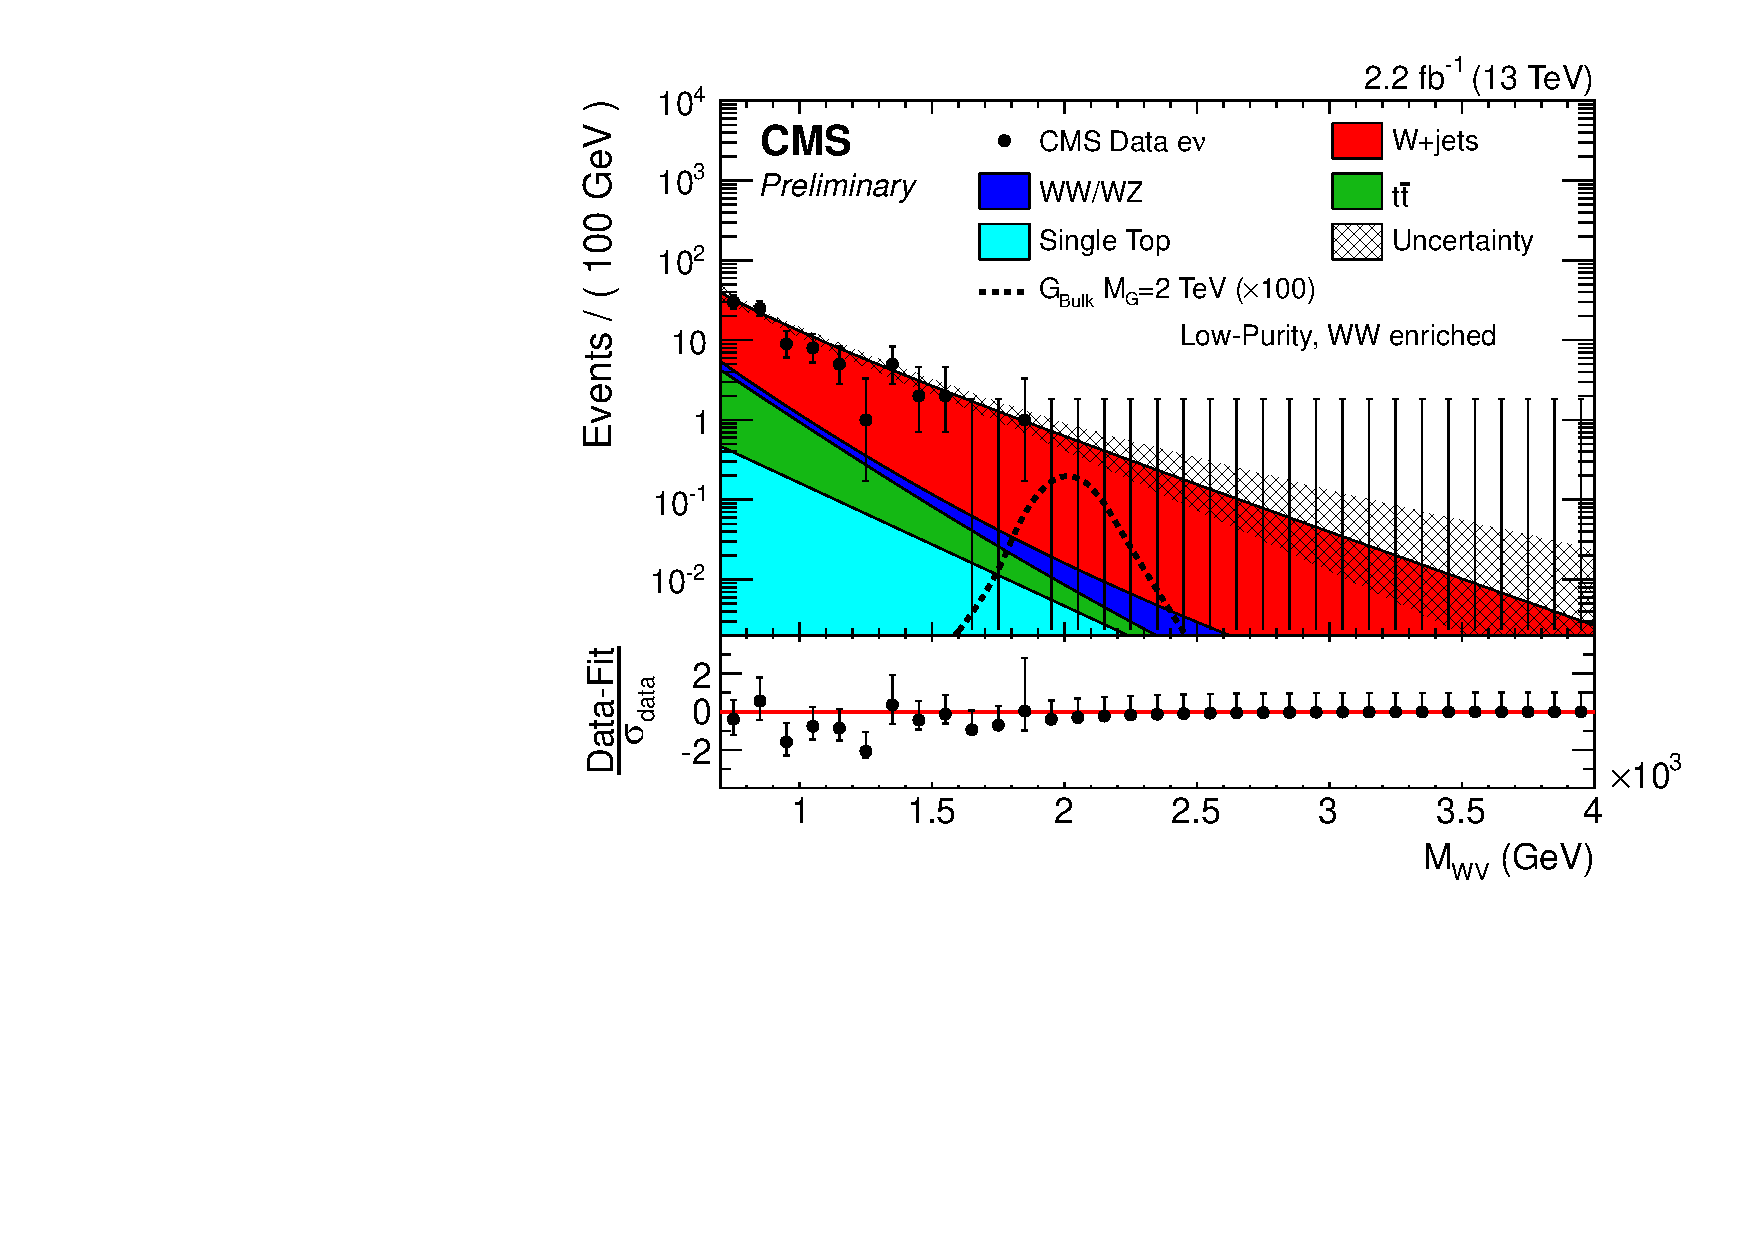
\includegraphics[width=0.48\textwidth]{\chtwelve/LPW_mlvj_fitting_el}\\
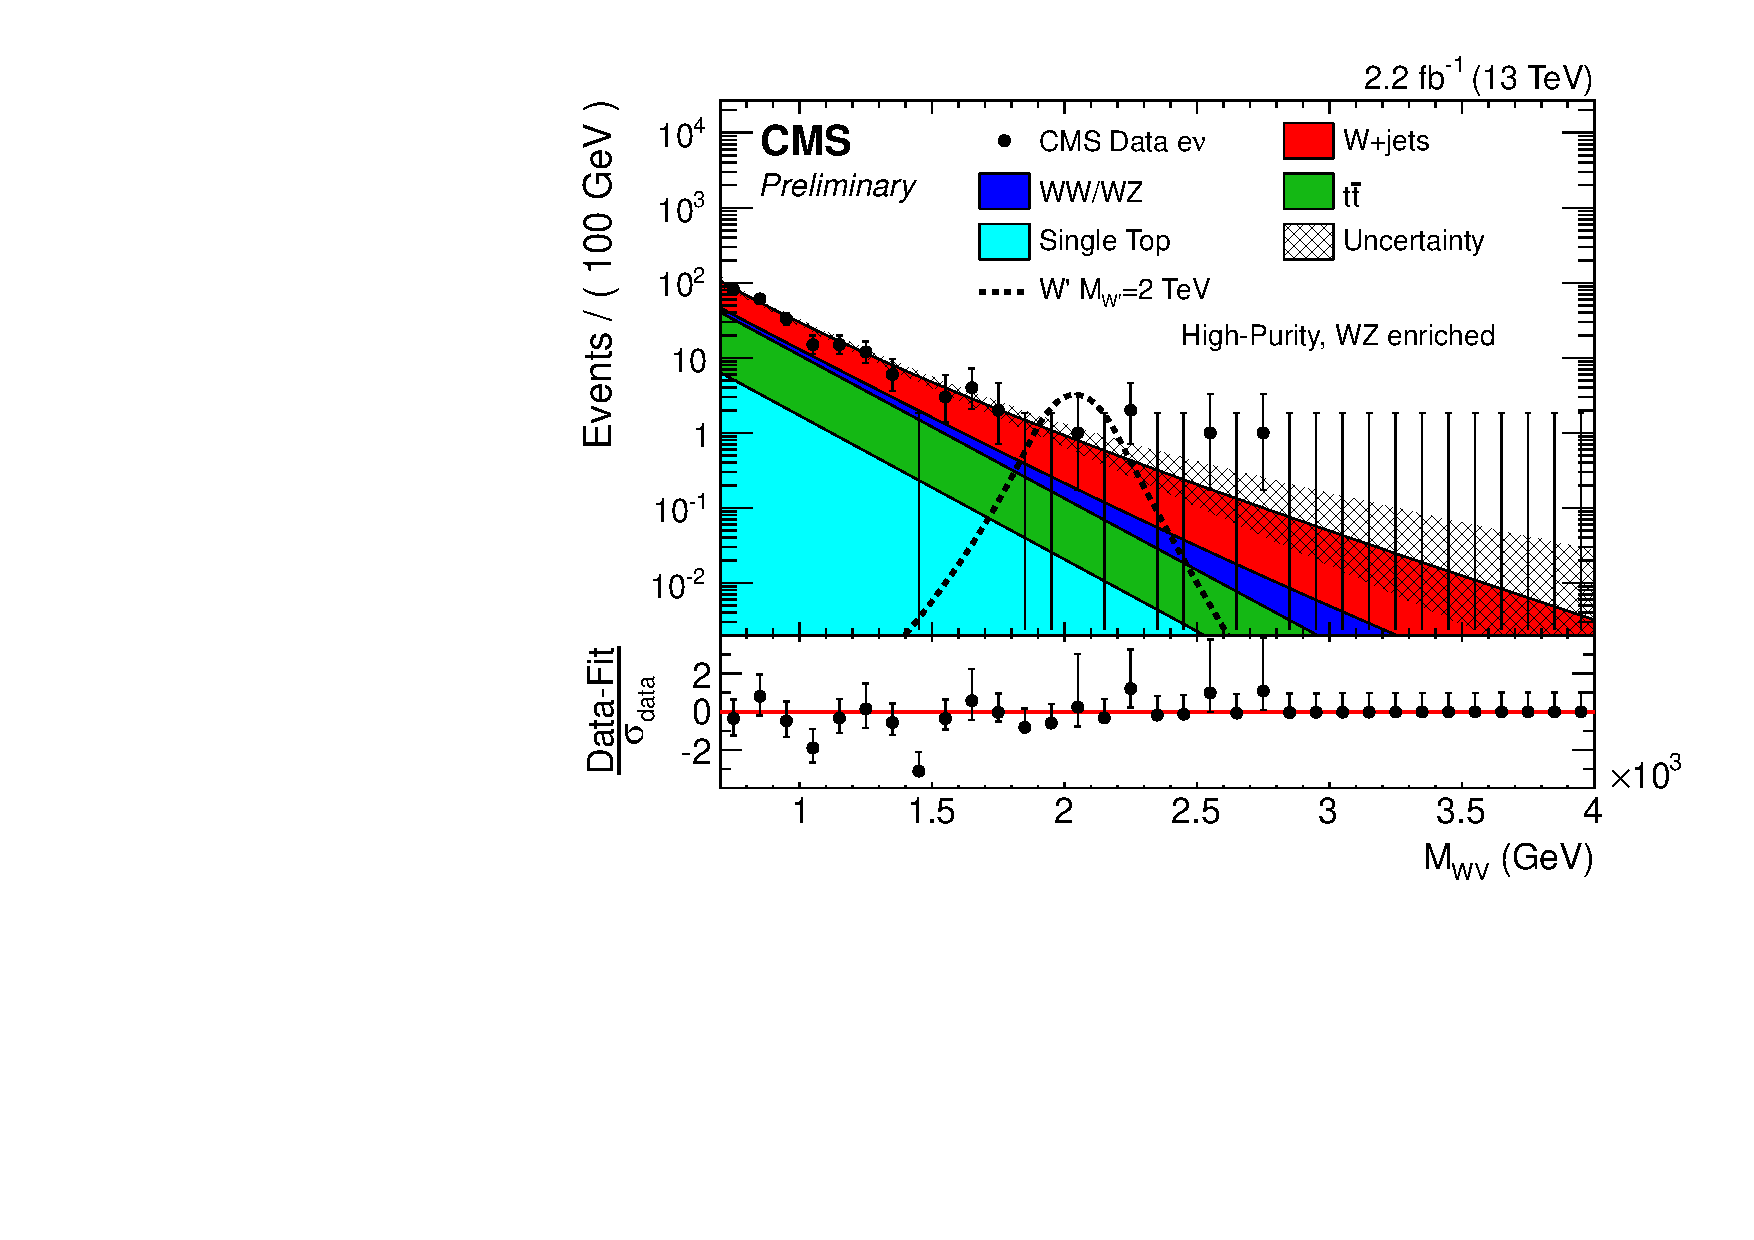
\includegraphics[width=0.48\textwidth]{\chtwelve/HPZ_mlvj_fitting_el}
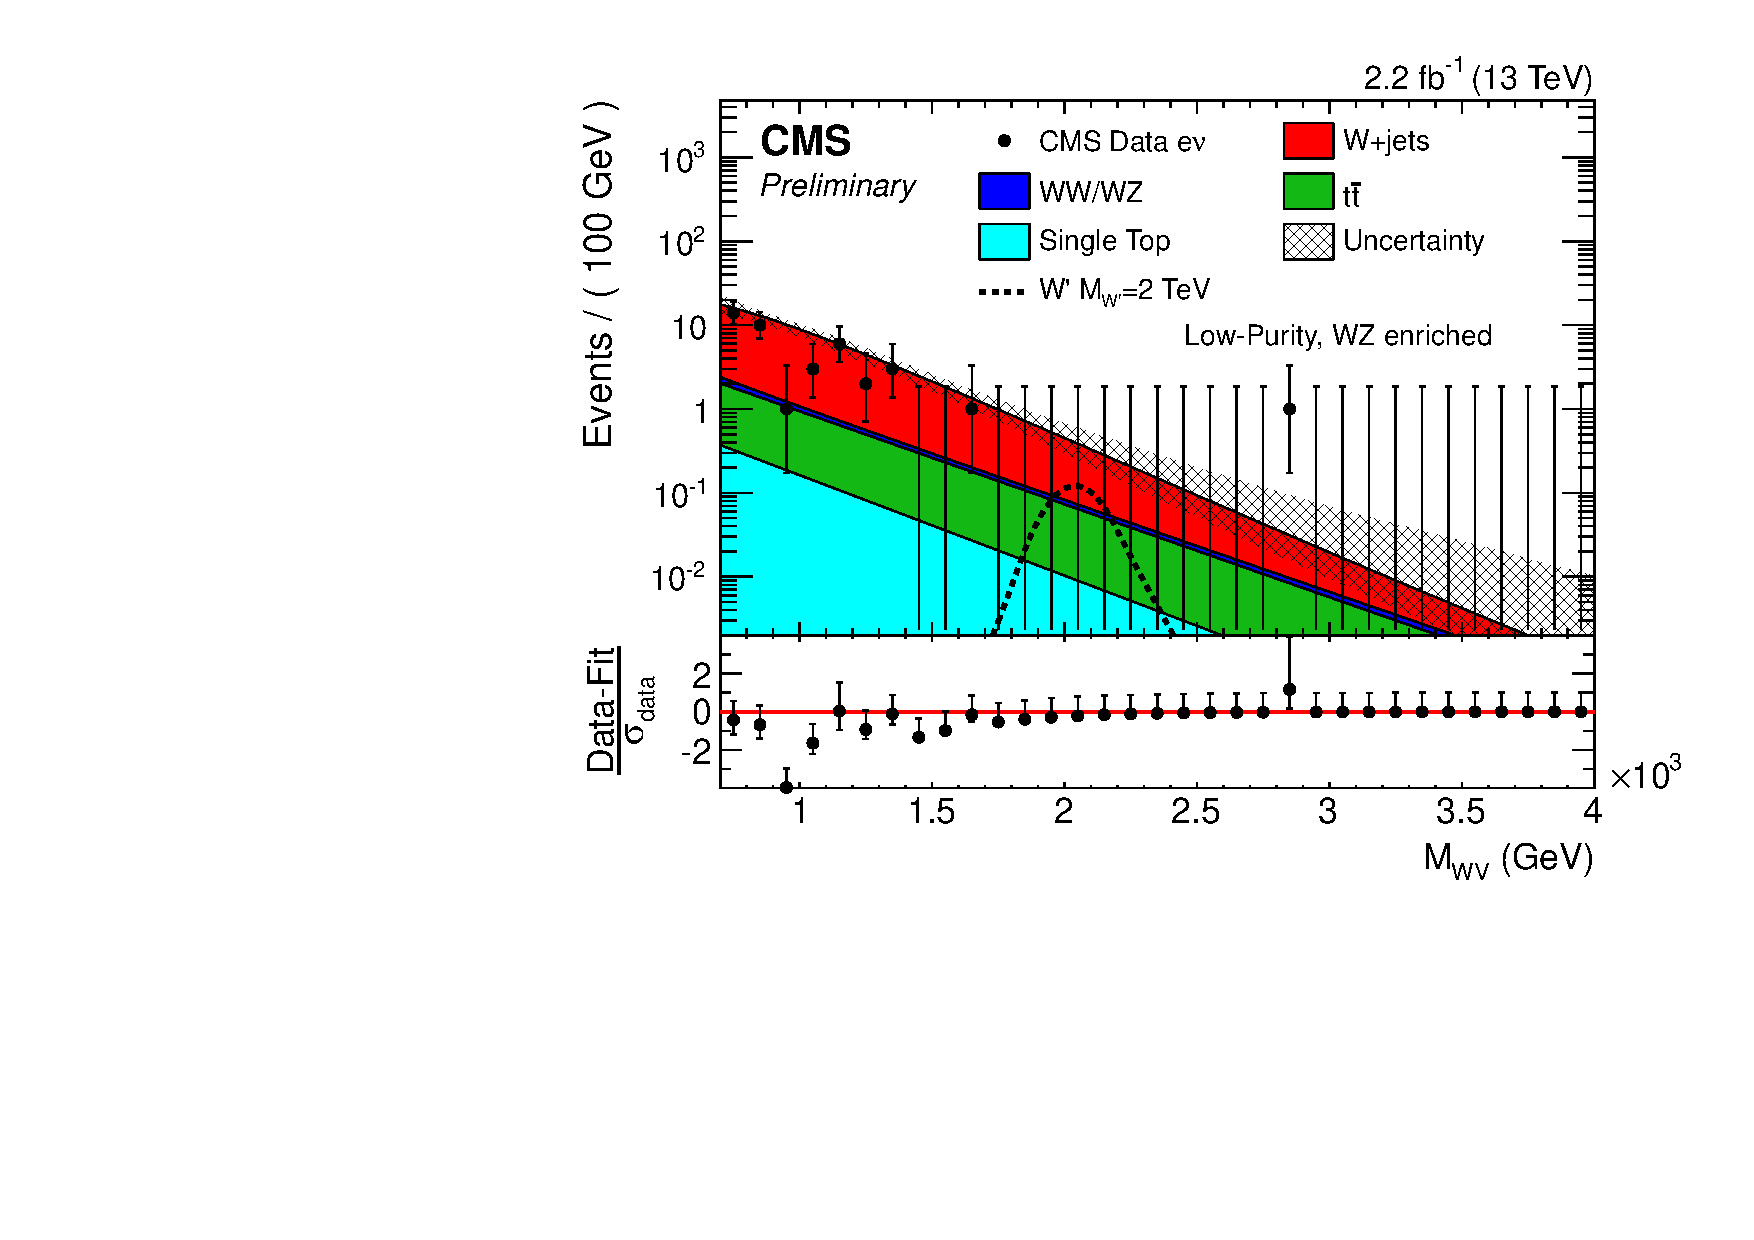
\includegraphics[width=0.48\textwidth]{\chtwelve/LPZ_mlvj_fitting_el}\\
\caption{Examples of $m_J$ extrapolation of the $m_{\ell\nu j}$ shape into the Signal Region
for the electron channel for the HP (left) and LP (right) categories in the WW (top) and WZ (bottom) signal regions.
The expected shape for a Bulk Graviton and for a W' with a mass of 2 TeV is also shown
in the WW-enriched and WZ-enriched category, respectively.}
\label{fig:srFits_el}
\end{figure}

\section{Cross section limits}

\begin{figure}[htbp]
\centering
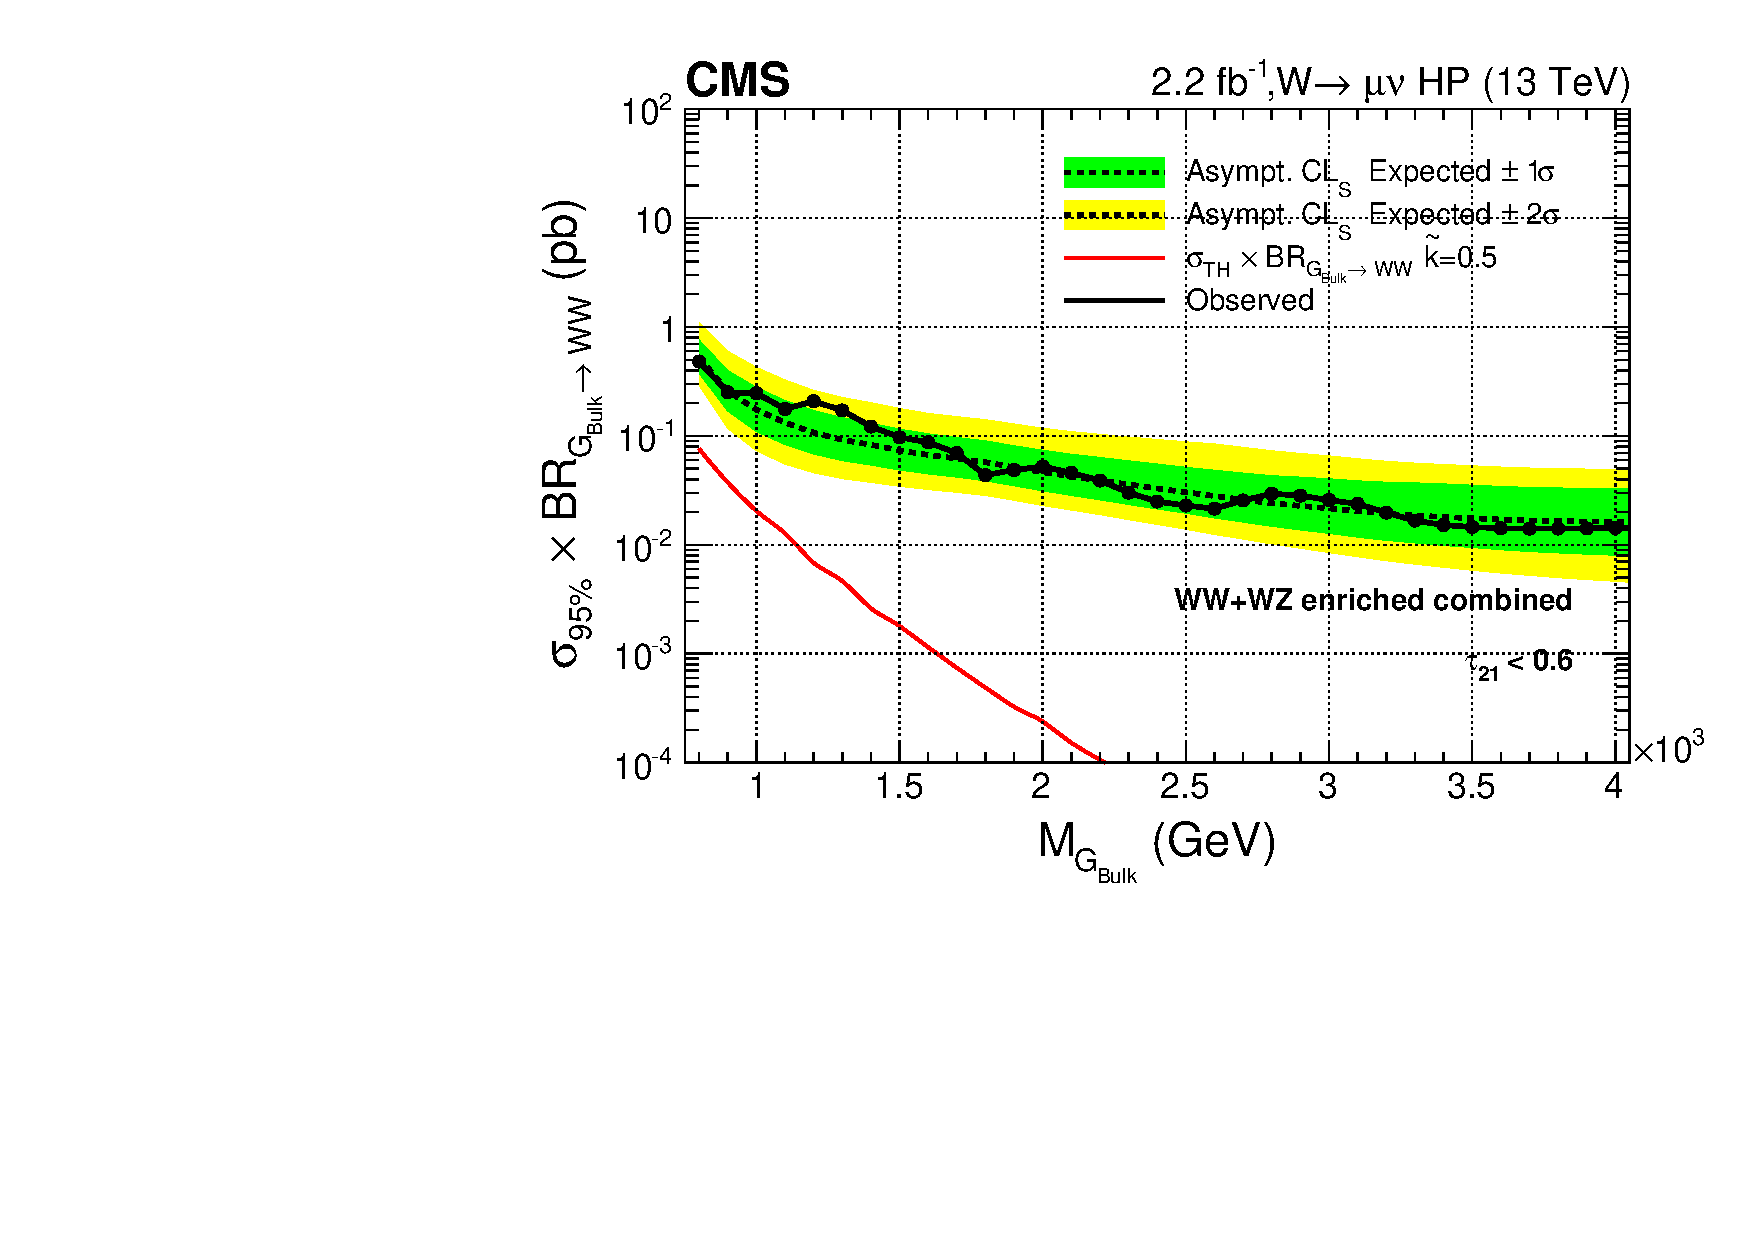
\includegraphics[width=0.48\textwidth]{\chtwelve/Lim_mu_HP_BulkG_WW.pdf}
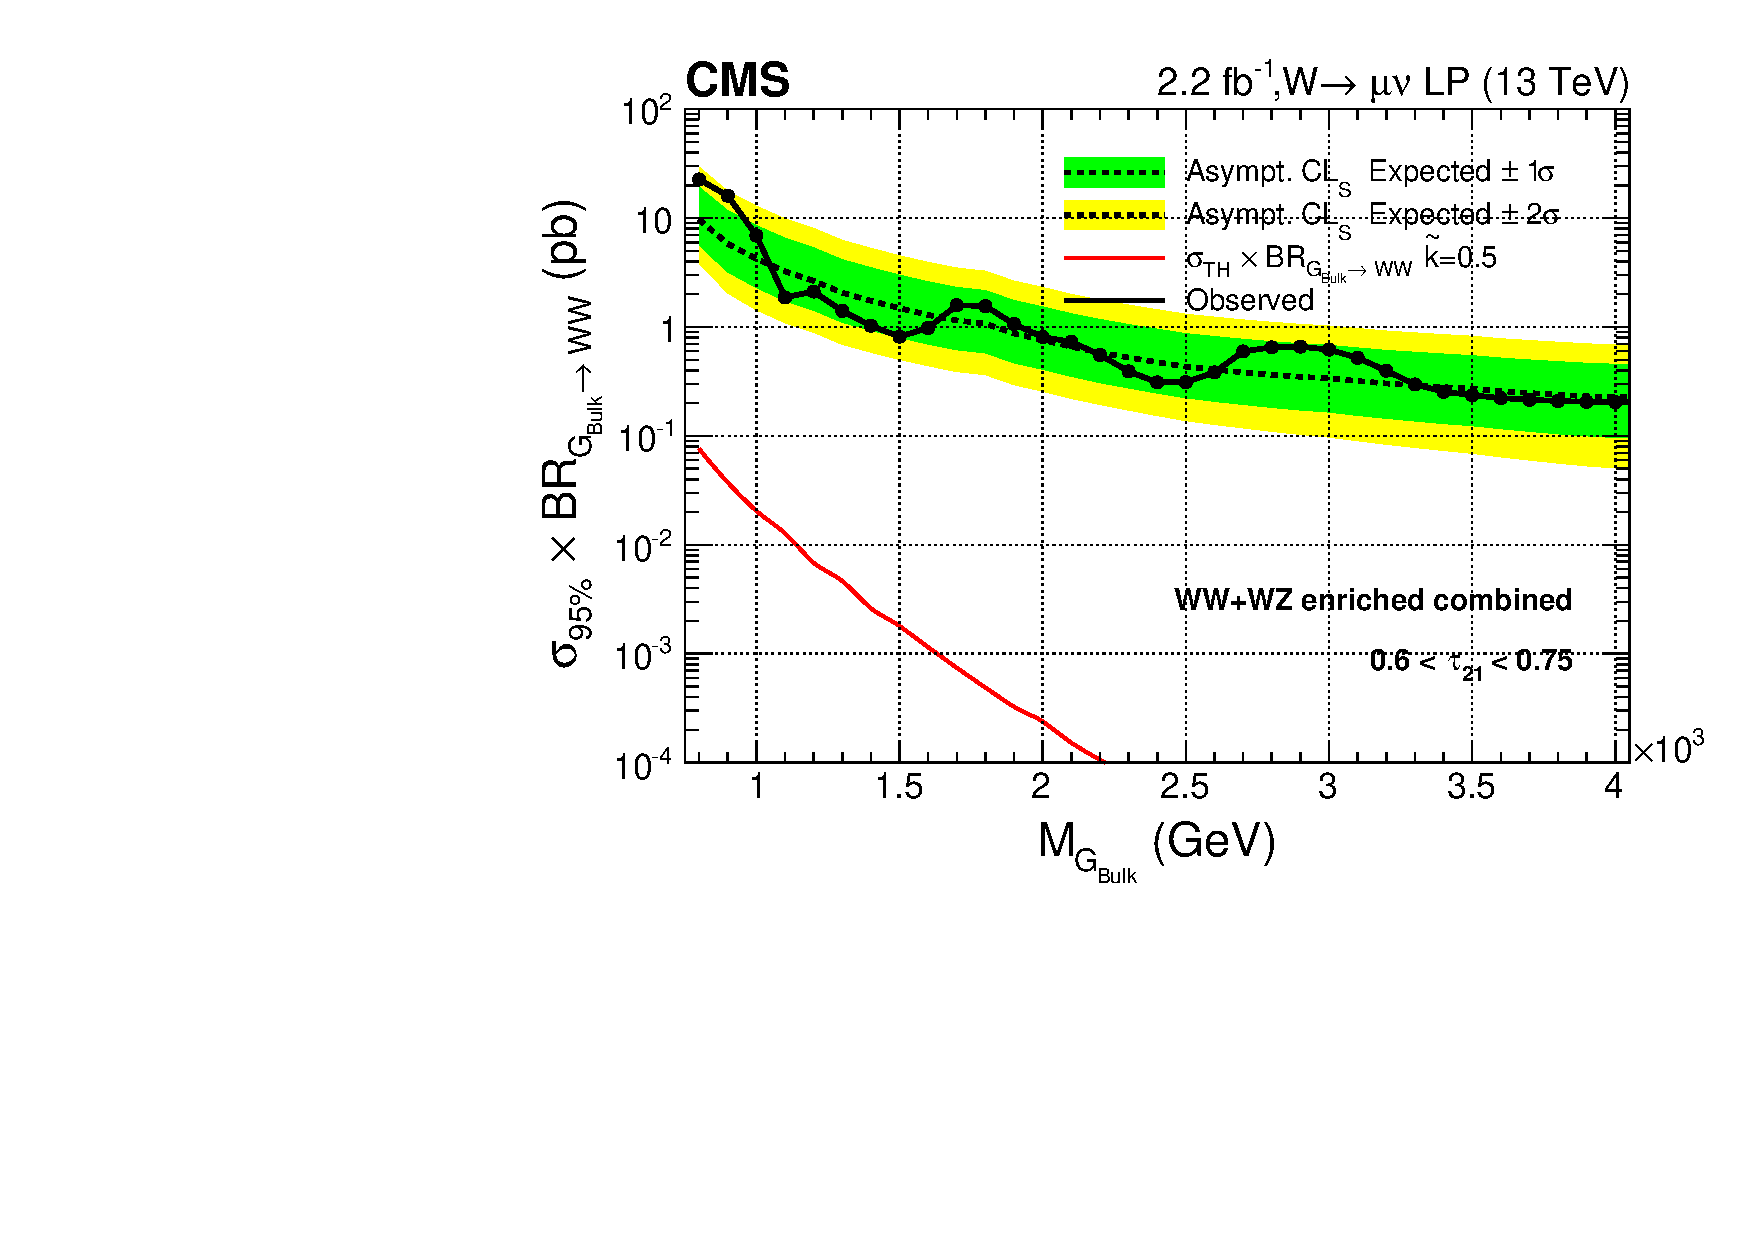
\includegraphics[width=0.48\textwidth]{\chtwelve/Lim_mu_LP_BulkG_WW.pdf}\\
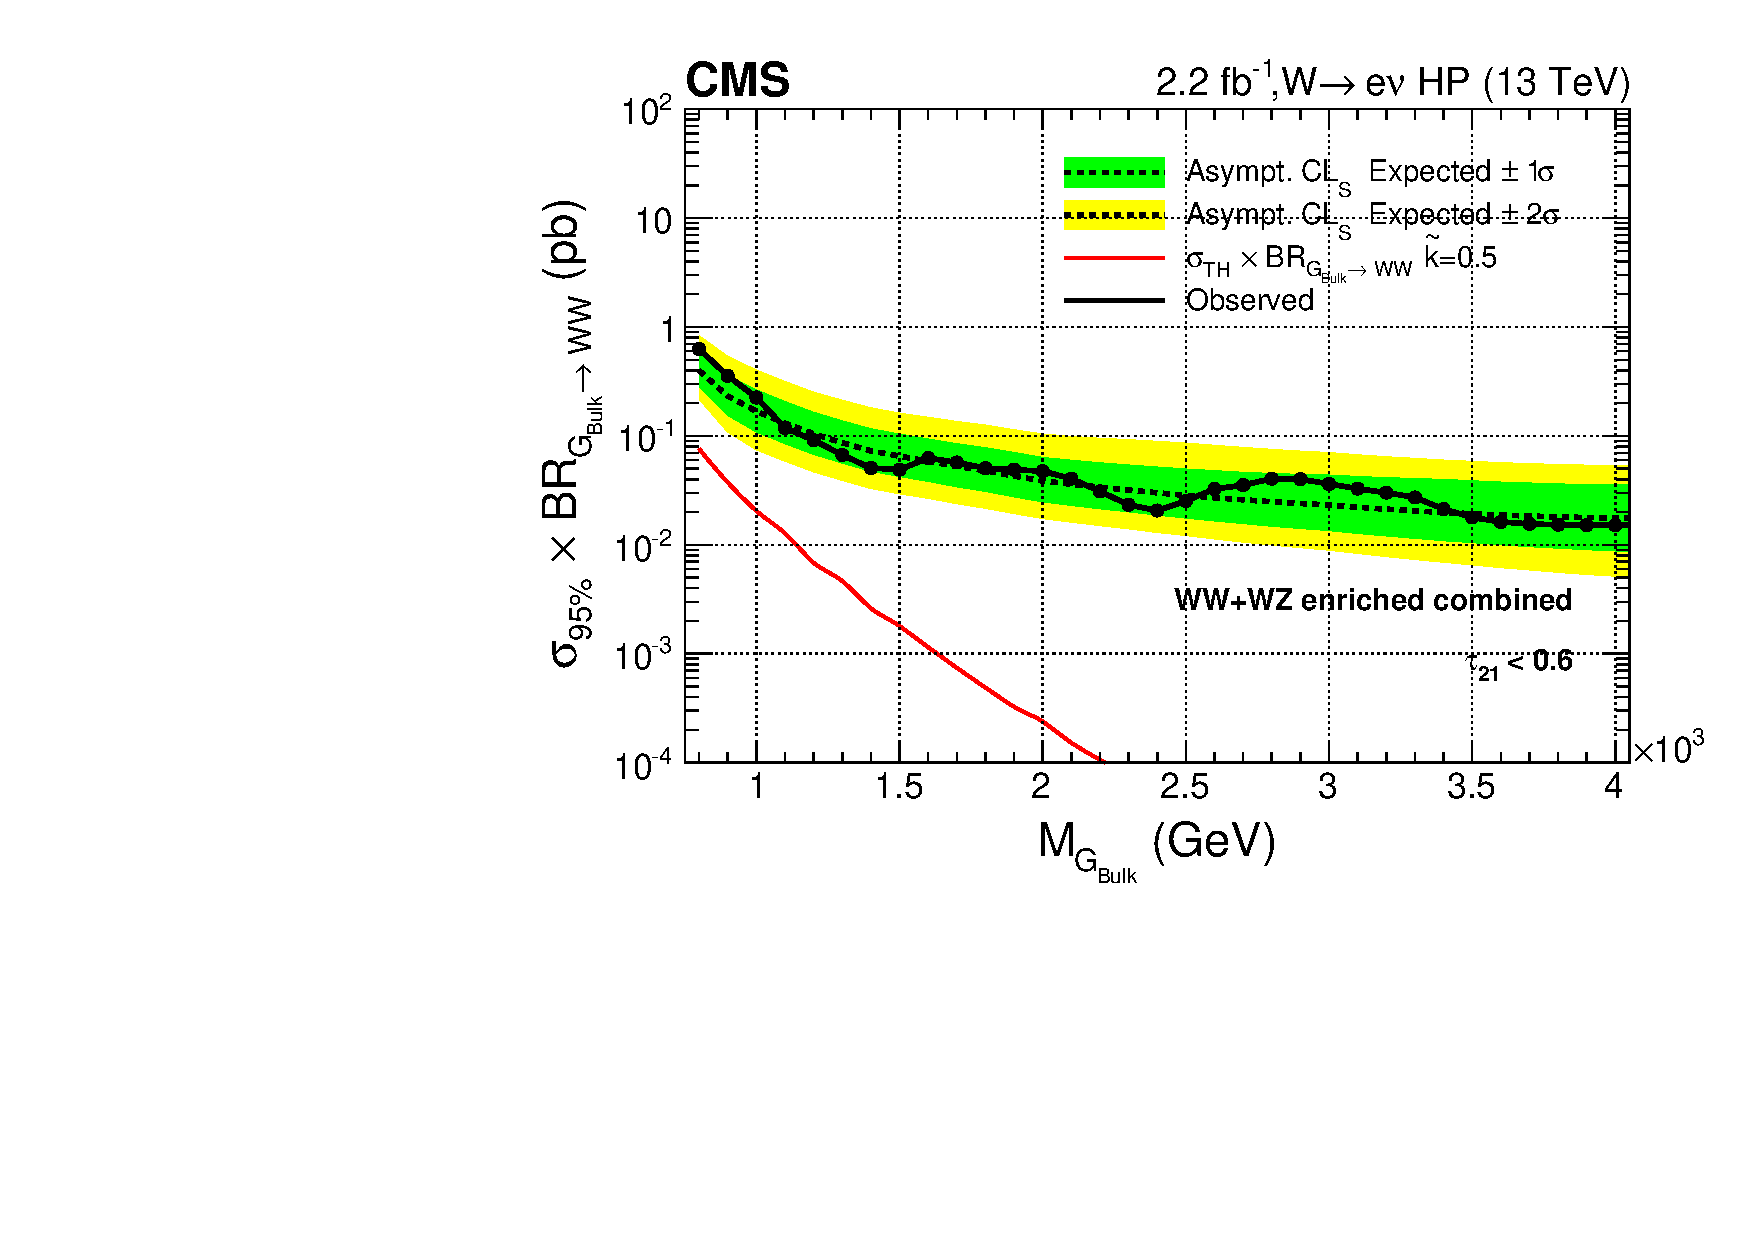
\includegraphics[width=0.48\textwidth]{\chtwelve/Lim_el_HP_BulkG_WW.pdf}
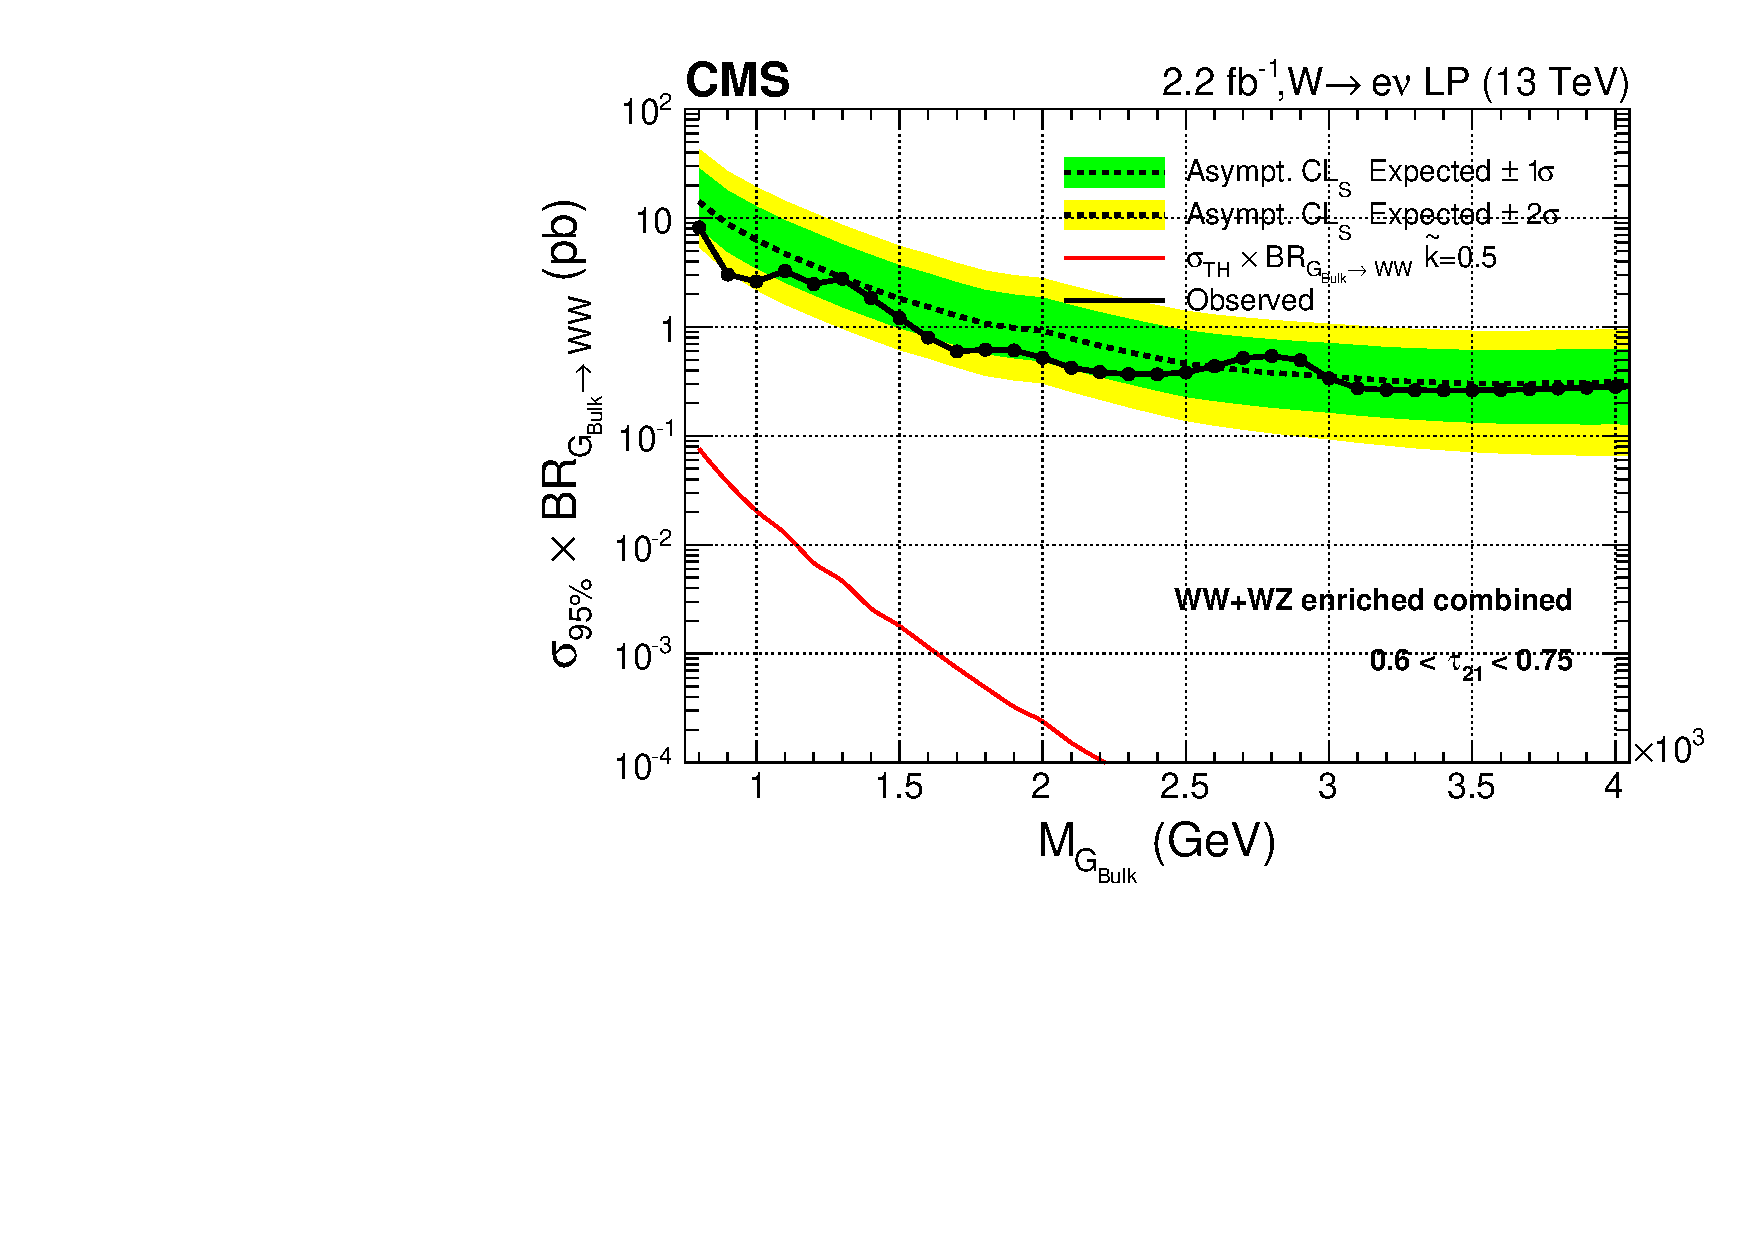
\includegraphics[width=0.48\textwidth]{\chtwelve/Lim_el_LP_BulkG_WW.pdf}\\
\caption{Expected 95\% CL upper limit on graviton production cross section times the branching fraction of $G_{bulk} \rightarrow WW$ assuming 2.1 fb$^{-1}$ of data. The limit is obtained with the Asymptotic CLs technique. The 68\% and 95\% ranges of expectation are
also shown with green and yellow bands. The expected product between the Bulk graviton
production cross section and the branching fraction is shown as a red solid curve for $\tilde{k} = 0.5$.
Top panel: results for muon channel, HP category on the left, LP on the right. Bottom panel: results for electron channel, HP category on the left, LP on the right.
}
\label{fig:limits_1}
\end{figure}

\begin{figure}[htbp]
\centering
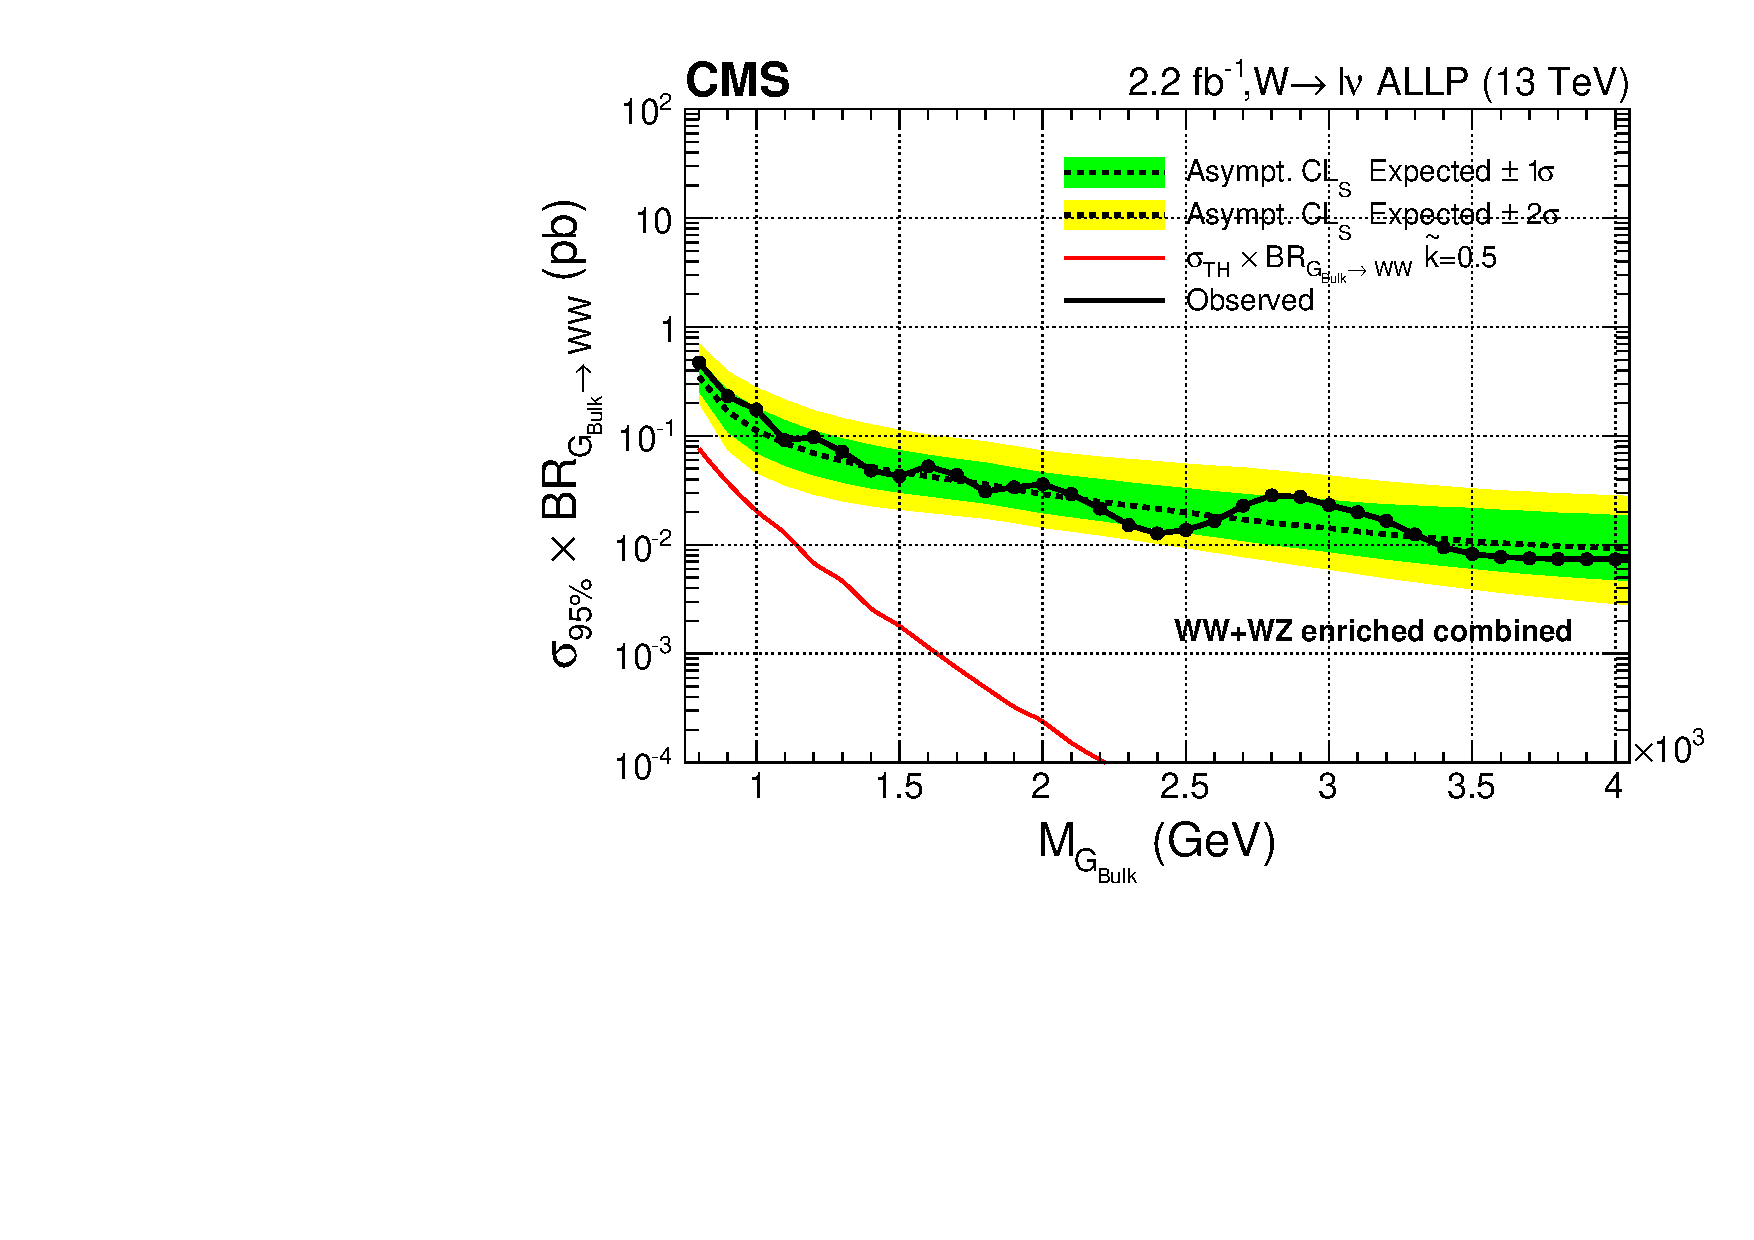
\includegraphics[width=0.5\textwidth]{\chtwelve/Lim_combo_ALLP_BulkG_WW.pdf}
\caption{Expected 95\% CL upper limit on the graviton production cross section times the branching fraction of $G_{bulk} \rightarrow WW$ assuming 2.1 fb$^{-1}$ of data. The limit is obtained with the Asymptotic CLs technique. The 68\% and 95\% ranges of expectation are also shown with green and yellow bands. The expected product between the Bulk graviton production cross section and the branching fraction is shown as a red solid curve for $\tilde{k} = 0.1$.}
\label{fig:limits_2}
\end{figure}

%\chapter{Statistical and model interpretation}
%\label{ch:limits}

%\section{Testing new resonance hypothesis}
%\subsection{Profile likelihood procedure}
%\subsection{The CL$_{s}$ method}
%\subsection{Treatment of uncertainties}

%\section{Limits on the 8 and 13 TeV cross sections}
